\chapter{Asking A 27 Year Old How to Make \$300 Million}

This lecture is an interview, not a blackboard performance, but it still unfolds with a definite analytic order. We begin with scale, then rewind to origin, then ask what structural change separates seven, eight, and nine figures. From there the lecture pivots outward: first from firm architecture to personal escape from poverty, then from location to relationships, and finally from income to capital deployment, sales conviction, and the lecturer's own distinction between being rich and being wealthy. Since no validated board figures survive for this chapter, the displayed formulas and diagrams below are transcript-derived compressions of the spoken argument rather than transcriptions of visible mathematics.

\section{Scale Shock, Then Rewind}

The lecture opens exactly where it wants our attention to be: on magnitude. Before we know the method, we are told the scale of the result. The company reportedly did about \$149 million in the prior year and is on track for roughly \$300 million in the present one:
\begin{align}
R_{\text{last}} &= \$149\text{M},\\
R_{\text{proj}} &\approx \$300\text{M}.
\end{align}
So the opening claim is not merely that the company is large; it is that the business is moving at something like a doubling rate:
\begin{equation}
g=\frac{R_{\text{proj}}}{R_{\text{last}}}\approx \frac{300}{149}\approx 2.0.
\end{equation}
We should keep the source discipline here. These are company-scale revenue figures, not clearly stated personal earnings, even though the question is framed in personal terms.

Only after this cold open does the narration rewind. The speaker takes us back to poverty, immigrant parents, the decision to master sales, and the eventual move from salesperson to leader to owner. That rewind matters. It prevents the later business advice from floating free as generic self-help. We are meant to feel the present scale and then ask, step by step, what had to change in order to make such scale possible.

There is also a source-sensitive distinction to preserve. The narration briefly speaks in very large promotional language about one of the largest solar companies in the world, whereas the interview proper is more concrete: the firm is presented as one of the largest residential solar installers in the United States. The operational snapshot is specific enough to matter: more than 600 W2 employees, more than 3,000 sales reps selling through the firm, and a business already functioning at very substantial volume.

\section{The Seven-, Eight-, and Nine-Figure Thresholds}

The first serious mechanism in the lecture appears when the interviewer asks what actually carries a company from seven to eight to nine figures. Here the lecture stops being merely biographical. It becomes structural. The answer is a threshold model.

A compact way to encode the spoken ladder is
\begin{align}
\mathcal{S}_7 &= \{\text{idea},\text{sales},\text{marketing}\},\\
\mathcal{S}_8 &= \mathcal{S}_7 \cup \{\text{team}\},\\
\mathcal{S}_9 &= \{\text{product},\text{marketing},\text{sales},\text{team},\text{systems}\}.
\end{align}
The transcript briefly stumbles and repeats part of the team line, but the intended progression is clear enough. Seven figures require a viable offer and the ability to move it. Eight figures require people. Nine figures require that the business cease to depend on improvisation and begin to depend on systems.

\begin{figure}[h]
\centering
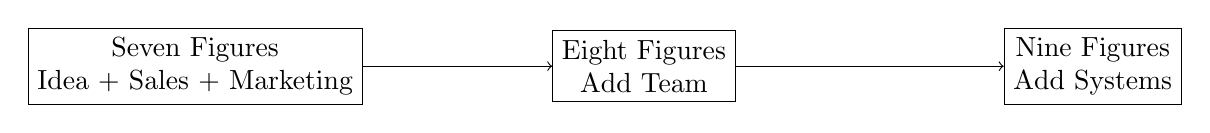
\begin{tikzpicture}
\node[draw, rectangle, align=center] (a) at (0,0) {Seven Figures\\Idea + Sales + Marketing};
\node[draw, rectangle, align=center] (b) at (5.7,0) {Eight Figures\\Add Team};
\node[draw, rectangle, align=center] (c) at (11.4,0) {Nine Figures\\Add Systems};
\draw[->] (a) -- (b);
\draw[->] (b) -- (c);
\end{tikzpicture}
\caption{Transcript-derived schematic of the lecture's scale thresholds.}
\end{figure}

What is important is not the labels by themselves, but the change in what constrains the firm. The lecture does not say that one simply works harder and climbs. It says that each scale has a dominant bottleneck, and the next scale appears only when that bottleneck is removed.

\subsection{Question \& Answer}

\paragraph{Question.} Why do firms so often stall between eight figures and nine figures?

\paragraph{Answer.} Because the eight-figure firm can still be secretly organized around the founder. It may have activity, sales, and a real team, but key functions still terminate in one person. The nine-figure transition occurs when the business becomes executable through procedures rather than personality.

We can formalize the lecture's operational intuition.

\begin{definition}
A business is founder-dependent if there exists a critical function \(f\) for which the founder, or a single irreplaceable operator, remains the unique reliable executor.
\end{definition}

Let \(D(f)\in\{0,1\}\) denote whether a function \(f\) has been documented in a usable standard operating procedure. Then the lecture's claim is that documentation changes the continuity structure of the business:
\begin{equation}
D(f)=1 \;\Rightarrow\; \exists\,c\neq o \text{ such that } c \text{ can execute } f,
\end{equation}
where \(o\) is the original operator and \(c\) is a colleague.

\begin{proposition}
As documentation coverage across critical functions rises, founder dependence falls.
\end{proposition}

\begin{proof}
If a critical function is not documented, then the absence of the founder or original operator can halt that function entirely. Once the function is documented in a form another colleague can use, execution can survive the founder's absence. Repeating this across many functions transfers continuity from the person to the machine of the business. This is precisely the lecture's contrast between an eight-figure firm that still relies on the CEO and a nine-figure firm that relies on systems.
\end{proof}

So we obtain a clean monotonic statement:
\begin{equation}
D_{\text{coverage}}\uparrow \;\Rightarrow\; \text{founder dependence}\downarrow.
\end{equation}
The lecture pushes this logic to its sharpest edge: if the founder disappears, does the business merely survive, or does it continue to scale? That is the test of whether the organization is still centered on the founder or has become a machine.

\section{Escaping Poverty by Changing Environment}

Once the lecture has described how a business escapes founder-bottleneck, it turns to a different bottleneck altogether: poverty. The interviewer asks what someone trapped in the cycle of poverty should do. The answer is not simply ``work hard.'' The answer is that environment changes what one sees, whom one can meet, and what level of life feels imaginable.

A cautious summary of the heuristic is
\begin{equation}
E[\text{opportunity access}] \propto \rho_{\text{wealth}}(\text{environment}),
\end{equation}
where \(\rho_{\text{wealth}}\) is a transcript-derived symbol for the local density of capital, wealthy actors, and visible economic motion. This is not an econometric law; it is the lecture's way of thinking. But it is central to the pacing of the interview.

The speaker makes the point through contrast. In one environment, everyone nearby earns ordinary wages, the surroundings are broken down, the social field is stagnant, and daily life presses downward on ambition. In another, one moves through a city full of expensive cars, celebrities, active businesses, visible capital, and fast economic circulation. In the lecture's view, that second environment does two things at once: it raises access and it raises appetite.

The interview gives a concrete, highly rhetorical example: in a major city, within a 30-mile radius, one might be near 14 billionaires and tens of thousands of multimillionaires. We should not treat these as audited demographic statistics. Their role is not statistical certification; their role is to model density. The point is that in one place one is near little money, and in another one is near enormous amounts of it. The probability of productive collisions changes.

There is a hidden symmetry here with the earlier business discussion. In the scale section, the bottleneck was the founder. In the poverty section, the bottleneck is the environment itself. In both cases the lecture wants us to stop talking about willpower in the abstract and start asking where the binding constraint actually lives.

\subsection{Question \& Answer}

\paragraph{Question.} If the obstacle is poverty, what should a young person invest in first?

\paragraph{Answer.} First, invest in escape velocity itself: build skill, save money, and move. The lecture is explicit that prestige spending is not the first answer, and neither, in the early stage, is passive investing in things like real estate or the stock market.

The priority rule can be written schematically as
\begin{equation}
\text{if trapped, then } \quad H + P \succ A_{\text{passive}},
\end{equation}
where \(H\) is human capital, \(P\) is positional leverage created by relocation, and \(A_{\text{passive}}\) denotes early passive asset accumulation.

A slightly more granular version of the lecture's ordering is
\begin{equation}
\text{priority}=
\begin{cases}
\text{build skills}, & \text{if one is too young to move},\\
\text{save and relocate}, & \text{if mobility is possible},\\
\text{add passive investing later}, & \text{after earnings power improves}.
\end{cases}
\end{equation}
This is not financial orthodoxy stated from nowhere. It is a theory of escape from a bad basin of attraction.

\section{Invest First in Self, Then in Position}

The next movement of the lecture is not really a new thesis; it is the operational completion of the previous one. Once the speaker has argued that environment matters, he turns that claim into a program. We are told to save money not for symbolic security, but for movement. We are told to buy skills before we buy status. We are told to become a closer, a marketer, a salesperson, a person who can generate cash in many environments.

The spoken ordering is concrete enough to preserve:
\begin{enumerate}
\item build monetizable skill, especially in sales and marketing;
\item save enough money to change environment;
\item resist buying cars, watches, clothes, and other prestige symbols too early;
\item only then treat passive assets as a serious priority.
\end{enumerate}

The lecture is especially vivid when it turns from finance to morale. It says, in effect, that surroundings act as repeated inputs into ambition. If we walk outside into visible decay, we are pressed downward. If we walk outside into a city vibrating with money, deals, attention, and movement, we are pulled upward. This is why the lecture dwells so long on the difference between a dead environment and a live one. A careless summary would collapse all this into the slogan ``move to a better city.'' But the lecture's real point is more precise: environment changes both the opportunity set and the psychology with which we approach it.

\section{A Brief Pause, Then Relationships}

At this point the transcript pauses for a sponsor message. In the notes we keep the interruption only as a marker of pacing. The conceptual line is resumed afterward, but on a new axis. We now move from place to people.

The post-interruption question asks about the importance of surrounding oneself with the right people and about leveraging relationships in the business world. The answer is severe and clean. Successful people do not, as a rule, pour time and value into strangers who bring nothing. They are not necessarily cruel; they are simply allocating attention toward what matters in their own lives.

That is why the lecture treats networking as an exchange problem, not as a begging problem. A cautious schematic is
\begin{equation}
\text{access} \sim f(\text{value provided},\text{credibility},\text{trust}),
\end{equation}
where the symbol \(f\) names a qualitative relation rather than a measurable formula.

\subsection{Question \& Answer}

\paragraph{Question.} How do we build real networks if powerful people do not automatically help strangers?

\paragraph{Answer.} We do not begin by asking for rescue. We begin by becoming the kind of person who can enter a room without lowering its value. The invitation is not the first event. Self-construction is the first event.

This part of the lecture has a definite sequence:
\begin{enumerate}
\item build yourself until admission into better rooms becomes plausible;
\item when admitted, do not arrive as a petitioner asking for instant advice or rescue;
\item create value, or at least do not diminish the room;
\item be careful not only about whom you seek, but also about whom you continue to carry with you.
\end{enumerate}

The lecture presses this through a vivid thought experiment. Suppose one randomly meets a billionaire in the street, even a figure as visible as Elon Musk. One might get a moment, perhaps even a piece of content, but one does not thereby gain durable access. The encounter is not the capital. The prepared self is the capital.

The same logic explains the lecture's emphasis on negative company. The speaker says, in effect, that even if we ourselves are decent, our social orbit can lower how others price us. In that sense, networking is not merely about reaching upward. It is also about refusing the downward drag of a surrounding group that signals chaos, addiction, triviality, or lack of purpose.

\section{Capital at Work, Sales as Conviction, and the Meaning of Wealth}

The late lecture gathers several ideas that might look separate on first hearing: money, reinvestment, sales, and the distinction between rich and wealthy. But the unifying theme is productive force. What matters is not merely what one has, but whether what one has is working.

\subsection{Capital at Work}

The lecture's most provocative financial line is the instruction to spend money. This must be read carefully. The speaker is not praising careless consumption. He is opposing idle hoarding. If cash exceeds immediate operating needs, he wants it treated as something to deploy rather than admire.

A simple balance decomposition is
\begin{align}
K_{\text{bank}} &= K_{\text{ops}} + K_{\text{idle}},\\
K_{\text{idle}} &\mapsto K_{\text{deployed}}.
\end{align}
Here \(K_{\text{ops}}\) denotes what must remain to keep the business stable, while \(K_{\text{idle}}\) denotes surplus cash doing no work. The lecture's preference is then
\begin{equation}
K_{\text{idle}}\downarrow,\qquad K_{\text{deployed}}\uparrow.
\end{equation}

The speaker's analogy is a luxury car with no gasoline. It may be visually impressive, but it does not move. The more serious content is operational. Too much idle cash can make the business psychologically soft. Reinvestment, by contrast, both builds the principal asset and forces the organization to keep recreating value rather than resting on stored comfort.

\begin{remark}
This is a founder's growth doctrine, not a universal theorem of prudent finance. The lecture is arguing from the standpoint of a person whose dominant asset is the business and whose primary concern is scale.
\end{remark}

\subsection{Sales as Conviction}

The next movement is one of the cleanest in the whole interview. The speaker explicitly contrasts technique with belief and gives a rhetorical weighting:
\begin{equation}
\text{Sales effectiveness} \approx 0.9\,C + 0.1\,T,
\end{equation}
where \(C\) is conviction in the product and \(T\) is tactics, scripts, role plays, and objection handling.

Again, this is not a calibrated statistical model. It is a way of ranking causes. The lecture's claim is that conviction is the hidden state variable that buyers feel before they parse our formal technique.

We may write the logic in a short chain:
\begin{enumerate}
\item Buyers respond not only to words, but to tone, confidence, and belief.
\item Those signals are functions primarily of \(C\), not merely of \(T\).
\item Therefore polished technique without conviction may still produce weak conversion.
\item Conversely, a less polished seller with strong conviction may outperform a highly trained but inwardly doubtful one.
\end{enumerate}

This is why the lecture returns at the very end to sales as a life-changing skill. Sales is not treated merely as a job. It is treated as the study of human decision.

\subsection{Rich and Wealthy}

The final conceptual distinction in the lecture is between being rich and being wealthy. Here we must preserve the source-conscious warning: these are the speaker's personal categories, not canonical economic definitions. Still, they matter because they reveal how he scales ambition.

The interview's own vocabulary can be compressed as
\begin{equation}
\text{rich}\sim \$4\text{M}-\$10\text{M}/\text{yr},\qquad \text{wealthy}\gtrsim \$1\text{B}.
\end{equation}
The point is not merely numerical inflation. The point is asset depth. Wealth, in the lecture, means that one's money is so extensively deployed, and one's balance sheet so thick, that even extravagant purchases do not meaningfully wound the whole.

The worked example of the chapter comes from the yacht comparison. Suppose the net worth is \$100 million and the contemplated yacht costs \$50 million, with annual operating cost above \$12 million. Then the carrying burden alone is
\begin{equation}
\frac{\$12\text{M}}{\$100\text{M}}=0.12.
\end{equation}
So a single nonproductive luxury asset can consume roughly \(12\%\) of net worth per year in operating cost. The lecture uses this to argue that a headline number, even a large one, may still be fragile if the capital structure is too thin and too exposed to toys that do not generate additional value.

\subsection{Final Compression}

The interview closes by collapsing everything into two maxims: learn sales and never give up. By the time we reach this point, these lines no longer sound like ordinary motivation. They have acquired structure.

Learning sales means learning how value is communicated, how trust forms, and how one human being moves another to decision. Never giving up means persisting through successive bottlenecks: the poverty bottleneck, the environmental bottleneck, the founder bottleneck, the network bottleneck, and the capital-allocation bottleneck. The lecture's closing force lies precisely in this compression. It returns from many mechanisms to two final imperatives.

\section{Summary}

The lecture unfolds as a sequence of threshold arguments. It begins with scale shock, then rewinds to early scarcity so that the later claims feel earned rather than generic. We are then given the first major mechanism: seven figures demand an offer and the ability to sell it, eight figures demand a team, and nine figures demand systems that reduce founder dependence. From there the lecture pivots outward. Escaping poverty is treated as a problem of environment as well as effort, so early investment is directed toward skill, saving, and relocation rather than status goods or premature passive investing. After a brief sponsor interruption, the discussion turns to networking, where access is framed as a consequence of value rather than a gift to the unprepared. Finally, the lecture gathers its late themes: idle cash should be deployed, sales is driven primarily by conviction, and wealth is defined not by a flattering headline number but by the depth and resilience of deployed assets.

The numerical anchors remain important throughout: roughly \$149 million in prior-year company revenue, roughly \$300 million projected, a growth multiple of about \(2\), the rhetorical \(90/10\) split between conviction and technique, and the \(12\%\) annual carrying-burden example in the yacht discussion. But the deeper lesson is not merely numerical. The lecture's real subject is the organization of compounding force: systems in the firm, energy in the environment, credibility in relationships, deployment in capital, and conviction in sales.